 \subsection{Visualize the list of live runs}
Into the page of \emph{Track4Run} a User can visualize the list of live runs that can be followed online.

\begin{table}[H]
	\centering
    
    \begin{tabular}{|p{3.5cm}|p{10.3cm}|}
    
    \hline
    \textbf{\large{Actors}}  			& \tabitem User 	\\
    				 					
    \hline
    \textbf{\large{Goals}} 				& \ref{goal:run5}\\
    
    \hline
    \textbf{\large{Enter Condition}}	& The \emph{User} is already logged in.		\\
    
    \hline
    \textbf{\large{Events Flow}}		& \begin{enumerate}[leftmargin=0.5cm]
                                          	\item The \emph{User} selects the "Live Runs" button into the Track4Run page to visualize the list of live runs.
                                          	 \item The System shows the list of all the available live runs.
                                          \end{enumerate}
    										\\
    \hline
    \textbf{\large{Exit Conditions}}    & The list of live runs is shown.\\
    
    \hline
    \textbf{\large{Exceptions}} 		& There are no possible exceptions.\\
    
    \hline
    
    
    \end{tabular}
	
\end{table}

\begin{figure}[H]
    \centering
    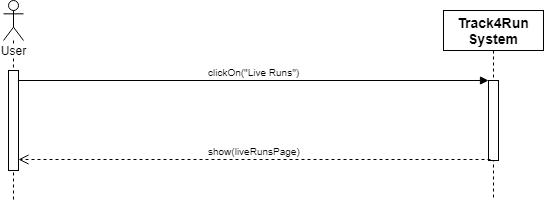
\includegraphics[scale=0.4]{Pictures/visListLiveRunsSeqDiag.png}
    \caption{Sequence diagram for the visualization of the list of live runs}
\end{figure}
